\documentclass[aspectratio=169,11pt]{beamer}

% Shared style (ib-tutorials.sty at the repo root).
\makeatletter\def\input@path{{./}{../}}\makeatother
\usepackage{ib-tutorials}

\usepackage[utf8]{inputenc}
\usepackage{amsmath,amssymb}
\usepackage{booktabs}
\usepackage{array}
\newcolumntype{L}[1]{>{\raggedright\arraybackslash}p{#1}}
\usepackage{graphicx}
\graphicspath{{../pictures/1-getting-set-up/}{pictures/1-getting-set-up/}}
\usepackage{xcolor}
\usepackage{listings}
\usepackage{tikz}
\usetikzlibrary{arrows.meta,positioning,shapes.geometric,fit,calc}
\usepackage{hyperref}

\newcommand{\sourcecredit}[1]{\vfill\hfill{\tiny\textcolor{DarkGray}{#1}}}

\lstset{
  basicstyle=\ttfamily\scriptsize\color{BlackGray},
  keywordstyle=\color{NavyBlue}\bfseries,
  commentstyle=\color{DarkGray}\itshape,
  stringstyle=\color{OliveGreen},
  showstringspaces=false,
  columns=fullflexible,
  keepspaces=true,
  frame=single,
  framerule=0.4pt,
  rulecolor=\color{LightGray},
  backgroundcolor=\color{LightGray!30},
  xleftmargin=0.25em,
  xrightmargin=0.25em
}
\lstdefinestyle{shell}{morecomment=[l]{\#}}
\lstdefinestyle{geo}{morecomment=[l]{//}}

\title[Software and geometries]{Choosing software and building geometries}
\subtitle{The CFD landscape, and how an organism becomes a mesh}
\author[Miller]{Laura A. Miller}
\institute[UArizona]{Department of Mathematics, University of Arizona}
\date{Using IB Software \textbullet\ Part I \textbullet\ Chapter 1b}

% pipeline boxes used on the title slide and on slide 10
\tikzset{pbox/.style={draw=DarkGray,rounded corners=1pt,fill=LightGray!45,text width=#1,align=center,inner sep=3pt,font=\scriptsize},
         pboxr/.style={draw=RubineRed,very thick,rounded corners=1pt,fill=RubineRed!8,text width=#1,align=center,inner sep=3pt,font=\scriptsize},
         parrow/.style={-{Stealth[length=2mm]},DarkGray}}

\begin{document}

% 1
\begin{frame}[plain]
\maketutorialtitlepanel{%
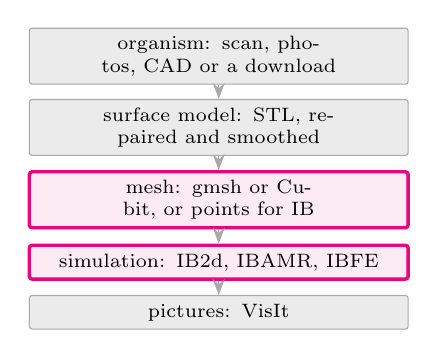
\begin{tikzpicture}[node distance=1.8mm]
  \node[pbox=46mm] (a) {organism: scan, photos, CAD or a download};
  \node[pbox=46mm,below=of a] (b) {surface model: STL, repaired and smoothed};
  \node[pboxr=46mm,below=of b] (c) {mesh: gmsh or Cubit, or points for IB};
  \node[pboxr=46mm,below=of c] (d) {simulation: IB2d, IBAMR, IBFE};
  \node[pbox=46mm,below=of d] (e) {pictures: VisIt};
  \foreach \p/\q in {a/b,b/c,c/d,d/e} \draw[parrow] (\p) -- (\q);
\end{tikzpicture}}
\end{frame}

% 2
\begin{frame}{Learning goals}
By the end of this chapter you should be able to:
\begin{enumerate}
  \item name the main open-source and commercial CFD codes, say what each is good for, and say where IB2d and IBAMR fit;
  \item explain why two codes, or two meshes, can give different answers for the same problem, and what to do about it;
  \item get a 3D model of an organism or object in four ways: download it, scan it, photograph it, or draw it;
  \item repair and smooth a surface so that a mesher accepts it, with tools that still exist;
  \item turn the surface into a volume mesh for IBFE, or an outline into points for IB2d and IBAMR, and check it before running.
\end{enumerate}
\vspace{3mm}
\begin{punchbox}
\small This chapter comes from the 2024 AIMEC--NSF Cassiopea workshop (``Software for Computational Fluid Dynamics, Part 1'') and from the geometry notes of the 2018--2022 courses. Chapter 18 goes into the meshers in detail; this chapter is the map.
\end{punchbox}
\end{frame}

% 3
\begin{frame}{Why simulate at all?}
\begin{columns}[T,onlytextwidth]
\begin{column}{0.55\textwidth}
\small Experiments show you the organism; simulations show you the \al{whole flow} and the \al{forces on every part}, and let you change things that nature does not:
\begin{itemize}
  \item the pressure and velocity inside a heart tube or around a wing, where no probe fits;
  \item the stiffness, shape, size or speed of the organism, one at a time;
  \item the Reynolds number, to ask what would happen if the animal were larger or the fluid thicker.
\end{itemize}
Two examples from the workshop: mosquito flight simulated from measured wing motion (Bomphrey et al.\ 2017), and jellyfish swimming driven by a neuromechanical model of the bell (Hoover et al.\ 2021).
\end{column}
\begin{column}{0.42\textwidth}
\begin{punchbox}
\small A simulation is a model. Its value lies in the question it answers and in the checks made along the way: does the answer change with the mesh, the time step, the box size, the boundary conditions? Chapters 8a, 16 and 4d are about those checks.
\end{punchbox}
\vspace{1mm}
\small An equation you can solve by hand describes a sphere, not a jellyfish: detailed models need numerical simulation.
\end{column}
\end{columns}
\end{frame}

% 4
\begin{frame}{Who does CFD now}
\begin{columns}[T,onlytextwidth]
\begin{column}{0.5\textwidth}
\textbf{Biologists}, with the codes in this chapter:
\begin{itemize}
  \item Eric Tytell (Tufts): swimming fish, and how the body and the flow push on each other.
  \item Lindsay Waldrop (Chapman): flows around the appendages of small crustaceans, in IB2d and IBAMR.
  \item Jake Socha (Virginia Tech): gliding snakes, with the Barba group's immersed boundary codes.
\end{itemize}
\end{column}
\begin{column}{0.48\textwidth}
\textbf{Undergraduates}, in one semester:
\begin{itemize}
  \item MATH 481 projects at the University of Arizona: for example, the flow through an embryonic heart built from a scan.
  \item An honors thesis at UNC on the flow around a scanned horseshoe crab, with IBFE.
\end{itemize}
\vspace{2mm}
\begin{punchbox}
\small The barrier is no longer the mathematics or the computer. It is knowing which tool to pick and how to get your organism into it, which is what the rest of this chapter is about.
\end{punchbox}
\end{column}
\end{columns}
\end{frame}

% 5
\begin{frame}{Open-source software}
\scriptsize
\begin{tabular}{@{}L{0.12\textwidth}L{0.1\textwidth}L{0.15\textwidth}L{0.11\textwidth}L{0.4\textwidth}@{}}
\toprule
Code & 2D/3D & Language, platforms & Re (rule of thumb) & Good for\\
\midrule
\al{IB2d} & 2D & MATLAB or Python; Linux, macOS, Windows & 0.01--1000 & learning the IB method; elastic, muscle-driven and porous boundaries; everything on a laptop (Part II)\\
\al{IBAMR} & 2D, 3D & C++; Linux, macOS (Windows through WSL2) & 0--5000 & elastic and rigid immersed bodies on adaptive grids; finite element solids (IBFE); clusters (Parts III--IV)\\
cuIBM, PetIBM & 2D (cuIBM), 2D and 3D (PetIBM) & C++ with GPUs; Linux & 0--5000 & rigid immersed bodies; PetIBM is the maintained successor of cuIBM (Barba group)\\
OpenFOAM & 2D, 3D & C++; Linux (macOS and Windows through containers or WSL2) & all, with the right solver & general-purpose finite volume CFD: pipes, turbulence, heat, multiphase; moving rigid bodies; a large user community\\
\bottomrule
\end{tabular}
\vspace{2mm}
\begin{itemize}
  \item The Reynolds-number ranges are the workshop's rules of thumb for what each code resolves comfortably: at higher Re the boundary layers get thin and the grid cost grows.
  \item IB2d and IBAMR share the same structure files, so a model built for one runs in the other (chapters 4a and 6).
\end{itemize}
\sourcecredit{IB2d: \url{https://github.com/nickabattista/IB2d}. IBAMR: \url{https://ibamr.github.io}. PetIBM: \url{https://github.com/barbagroup/PetIBM}. OpenFOAM: \url{https://openfoam.org}.}
\end{frame}

% 6
\begin{frame}{Commercial software}
\scriptsize
\begin{tabular}{@{}L{0.16\textwidth}L{0.19\textwidth}L{0.57\textwidth}@{}}
\toprule
Software & Platforms, cost & What it is\\
\midrule
COMSOL Multiphysics & Windows, macOS, Linux; license & finite elements for coupled physics (flow, heat, chemistry, structures) with a graphical workflow; a good match for complex geometries at low to moderate Re\\
ANSYS Fluent (now part of Synopsys) & Windows, Linux; license, free student version & finite volume CFD with meshing (Workbench); the Spring 2022 CFD course used it with scanned geometries\\
Autodesk CFD & Windows; education license & CFD inside the Autodesk CAD family\\
SimFlow & Windows, Linux; free limited version & a graphical front end for OpenFOAM\\
\bottomrule
\end{tabular}
\vspace{2mm}
\begin{itemize}
  \item These are not taught in these notes (chapter 0.1), but the geometry pipeline below is the same for all of them.
  \item Commercial meshers and post-processors are often the part people miss most when they move to open-source codes; gmsh and VisIt cover that ground here.
\end{itemize}
\sourcecredit{COMSOL: \url{https://www.comsol.com}. ANSYS: \url{https://www.ansys.com}. Autodesk CFD: \url{https://www.autodesk.com/products/cfd}. SimFlow: \url{https://sim-flow.com}.}
\end{frame}

% 7
\begin{frame}{Which one?}
\begin{columns}[T,onlytextwidth]
\begin{column}{0.55\textwidth}
\scriptsize
\begin{tabular}{@{}L{0.48\linewidth}L{0.44\linewidth}@{}}
\toprule
You want to \ldots & Start with\\
\midrule
learn how the IB method works, on a laptop & IB2d (Part II)\\
an elastic 2D organism, muscles, springs, a few hours per run & IB2d, then IBAMR for speed\\
3D, elastic solids, a cluster & IBAMR with IBFE (Parts III--IV)\\
a rigid, complicated shape at high Re & OpenFOAM, or a commercial code\\
many organisms in a given flow & Planktos on top of any of them (Part VI)\\
coupled heat, chemistry or electrics & COMSOL, or IBAMR's advection--diffusion (ch.\ 24)\\
\bottomrule
\end{tabular}
\end{column}
\begin{column}{0.43\textwidth}
\begin{punchbox}
\small Three questions decide most cases: Is the body elastic? Is it 2D or 3D? How thin are the boundary layers (how high is Re)? Elastic and 2D: IB2d. Elastic and 3D: IBFE. Rigid and high Re: a body-fitted finite volume code.
\end{punchbox}
\vspace{2mm}
\small Whatever you choose, the organism's geometry has to be built, cleaned and meshed first. That part is the same everywhere.
\end{column}
\end{columns}
\end{frame}

% 8
\begin{frame}{Does all software give the same answer?}
\begin{columns}[T,onlytextwidth]
\begin{column}{0.55\textwidth}
Mesnard and Barba (2017) tried to reproduce their own published result, the lift on the cross-section of a gliding snake at Re $= 2000$ and $35^\circ$, with four codes: cuIBM, PetIBM, IcoFOAM (OpenFOAM) and IBAMR.
\begin{itemize}
  \item The codes did \al{not} agree at first, and it took three years to understand why.
  \item Causes found: the outflow boundary condition and the box size; one bad triangle in a mesh, which made spurious vorticity; changes in the linear-algebra libraries between versions; how long the wake needs to become statistically steady.
  \item With those fixed, the results agreed, and the paper tells you exactly what was run.
\end{itemize}
\end{column}
\begin{column}{0.43\textwidth}
\begin{punchbox}
\small Lessons for every simulation in these notes: record the versions (chapter 0.2), check the box and the boundaries (chapter 7), check the mesh (this chapter and 18), and run long enough and fine enough to know what is converged (chapter 16).
\end{punchbox}
\vspace{2mm}
\small O. Mesnard and L. A. Barba, \emph{Reproducible and replicable CFD: it's harder than you think}, Computing in Science \& Engineering 19(4), 2017; \url{https://arxiv.org/abs/1605.04339}.
\end{column}
\end{columns}
\end{frame}

% 9
\begin{frame}{Mesh size matters}
\begin{columns}[T,onlytextwidth]
\begin{column}{0.55\textwidth}
The workshop deck showed the same snake wake on grids from $128^2$ to $4096^2$ cells (from the Barba group's flying-snake studies):
\begin{itemize}
  \item on the coarsest grids the wake is wrong in kind, not only in detail: the vortices are smeared and shed at the wrong times;
  \item the picture stops changing between the two finest grids, which is the sign that the result is \al{converged};
  \item the forces converge later than the pictures.
\end{itemize}
\vspace{1mm}
The same holds for the time step and for the number of points on an immersed boundary (chapter 5: about two points per grid cell).
\end{column}
\begin{column}{0.43\textwidth}
\begin{punchbox}
\small The rule: refine the grid (and the time step) until the quantity you care about stops changing, and report that quantity on at least two grids. Chapter 16 and the IB2d lab in chapter 4d show how.
\end{punchbox}
\vspace{2mm}
\small Adaptive refinement (IBAMR) puts the fine cells only where the boundary and the vortices are, which is why 3D is affordable at all (chapter 5).
\end{column}
\end{columns}
\end{frame}

% 10
\begin{frame}{From an organism to a simulation}
\centering
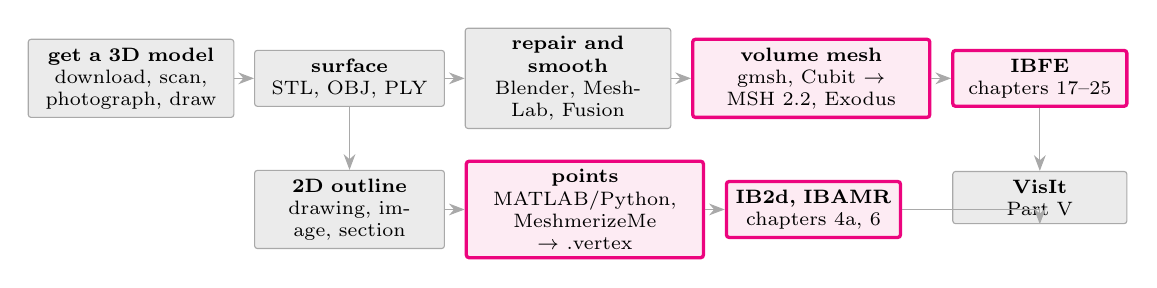
\begin{tikzpicture}[node distance=2.2mm and 2.5mm]
  \node[pbox=24mm] (acq) {\textbf{get a 3D model}\\download, scan, photograph, draw};
  \node[pbox=22mm,right=of acq] (surf) {\textbf{surface}\\STL, OBJ, PLY};
  \node[pbox=24mm,right=of surf] (rep) {\textbf{repair and smooth}\\Blender, MeshLab, Fusion};
  \node[pboxr=28mm,right=of rep] (vol) {\textbf{volume mesh}\\gmsh, Cubit $\to$ MSH 2.2, Exodus};
  \node[pboxr=20mm,right=of vol] (ibfe) {\textbf{IBFE}\\chapters 17--25};
  \node[pbox=22mm,below=8mm of surf] (out) {\textbf{2D outline}\\drawing, image, section};
  \node[pboxr=28mm,right=of out] (pts) {\textbf{points}\\MATLAB/Python, MeshmerizeMe $\to$ \code{.vertex}};
  \node[pboxr=20mm,right=of pts] (ib) {\textbf{IB2d, IBAMR}\\chapters 4a, 6};
  \node[pbox=20mm,below=8mm of ibfe] (viz) {\textbf{VisIt}\\Part V};
  \foreach \p/\q in {acq/surf,surf/rep,rep/vol,vol/ibfe,out/pts,pts/ib} \draw[parrow] (\p) -- (\q);
  \draw[parrow] (surf) -- (out);
  \draw[parrow] (ibfe) -- (viz);
  \draw[parrow] (ib) -| (viz);
\end{tikzpicture}
\vspace{3mm}
\begin{itemize}
  \item A 3D organism goes through the top row: a surface, cleaned, then filled with tetrahedra or hexahedra for IBFE.
  \item A 2D model needs only an outline and points along it, at about half a grid cell apart, for IB2d or IBAMR's IB method.
\end{itemize}
\end{frame}

% 11
\begin{frame}{Four ways to get a 3D model}
\scriptsize
\begin{tabular}{@{}L{0.12\textwidth}L{0.28\textwidth}L{0.26\textwidth}L{0.25\textwidth}@{}}
\toprule
Way & How & Good & Not so good\\
\midrule
Download & repositories of scanned specimens and drawn objects (next two slides) & minutes; museum CT scans are excellent & licenses; no units in STL; shapes may be artistic rather than accurate\\
Scan & structured-light or laser scanner, phone LiDAR app, micro-CT & real shape and size & small, shiny, wet or translucent organisms scan badly; holes and noise\\
Photograph & photogrammetry: 50--100 overlapping photos reconstructed into a surface & a camera is enough; works outdoors & needs care with light and overlap; no scale unless you add one\\
Draw & CAD: Tinkercad, Autodesk Fusion, FreeCAD, Blender, SolidWorks & clean, parametric, in real units; easy to vary & idealized; takes time to learn\\
\bottomrule
\end{tabular}
\vspace{2mm}
\begin{punchbox}
\small For a first simulation, draw a simplified organism in CAD. A clean, smooth shape in real units meshes in minutes; a raw scan can take days of repair, and the simulation will not resolve its finest details anyway.
\end{punchbox}
\end{frame}

% 12
\begin{frame}{Downloading: general repositories}
\begin{columns}[T,onlytextwidth]
\begin{column}{0.5\textwidth}
Sites with STL, OBJ and PLY files of everything from gears to animals, most made for 3D printing:
\begin{itemize}
  \item Thingiverse \url{https://www.thingiverse.com}
  \item Thangs \url{https://thangs.com}
  \item YouMagine \url{https://youmagine.com}
  \item Pinshape \url{https://pinshape.com}
  \item Sketchfab \url{https://sketchfab.com}
  \item Yeggi (a search engine) \url{https://www.yeggi.com}
  \item Libre3D \url{https://libre3d.com}
  \item GrabCAD (engineering parts; account needed) \url{https://grabcad.com}
\end{itemize}
\end{column}
\begin{column}{0.47\textwidth}
\begin{punchbox}
\small Check three things before you use a file: its \al{license} (many are Creative Commons, some non-commercial, some not for redistribution; these notes do not ship purchased models); its \al{units}, since STL has none, so measure a known length after import; and its \al{accuracy}, since a printable model is often simplified or stylized.
\end{punchbox}
\vspace{2mm}
\small Links checked in October 2026; sites come and go.
\end{column}
\end{columns}
\end{frame}

% 13
\begin{frame}{Downloading: scientific repositories}
\scriptsize
\begin{tabular}{@{}L{0.19\textwidth}L{0.4\textwidth}L{0.34\textwidth}@{}}
\toprule
Repository & What it holds & Link\\
\midrule
NIH 3D (formerly the NIH 3D Print Exchange) & anatomy, prostheses, proteins (``molecule of the month''), a heart library; scientifically accurate STL files & \url{https://3d.nih.gov}\\
MorphoSource & CT and surface scans of museum specimens worldwide; registration, and permission for some & \url{https://www.morphosource.org}\\
DigiMorph & high-resolution X-ray CT of biological specimens (University of Texas) & \url{http://www.digimorph.org}\\
Phenome10K & CT and surface scans of biological and palaeontological specimens, for academic use & \url{https://www.phenome10k.org}\\
GB3D Type Fossils & type specimens of British macrofossils & \url{https://www.3d-fossils.ac.uk}\\
Smithsonian 3D & scanned objects from the Smithsonian collections & \url{https://3d.si.edu}\\
UMORF & fossils from the University of Michigan Museum of Paleontology & \url{https://umorf.ummp.lsa.umich.edu}\\
\bottomrule
\end{tabular}
\vspace{2mm}
\begin{itemize}
  \item Many of these give you a \al{CT image stack}, not a surface. Segment it (mark the organism in the slices) in 3D Slicer, which is free, and export the surface as STL. \url{https://www.slicer.org}
  \item Scanned specimens come with their units; keep them when you export.
\end{itemize}
\end{frame}

% 14
\begin{frame}{Scanning}
\begin{columns}[T,onlytextwidth]
\begin{column}{0.5\textwidth}
\begin{itemize}
  \item \al{Structured-light and laser scanners} (makerspaces have them; MATH 762 used the UNC makerspace in 2019): sub-millimeter accuracy for objects from a few centimeters up; export OBJ, PLY or STL.
  \item \al{Phone apps} with LiDAR or photogrammetry (3D Scanner App, Polycam, Scaniverse): fast, for decimeter-sized objects, with rougher surfaces.
  \item \al{Micro-CT} for small organisms and for anything hollow or soft: a stack of slices, segmented into a surface (3D Slicer).
\end{itemize}
\end{column}
\begin{column}{0.47\textwidth}
\begin{punchbox}
\small Scan with a ruler or a calibration object in view, so that the scale can be checked. Shiny, dark, wet or translucent surfaces confuse optical scanners: dust them with powder, or use CT.
\end{punchbox}
\end{column}
\end{columns}
\end{frame}

% 14b
\begin{frame}{Scanning: what you get back}
\begin{itemize}
  \item The output is a \al{raw surface}: expect holes where the scanner could not see, floating fragments, duplicated and noisy patches, and a few million triangles. The repair step (slides 18--20) is not optional.
  \item Scanners export OBJ or PLY (with colors) or STL; CT gives DICOM slices that 3D Slicer segments into a surface and exports as STL.
  \item Keep the scanner's units when you export, and write them down: STL files do not carry them.
  \item A scan of a live or preserved animal is a snapshot of one posture; for a moving organism (a swimming jellyfish, a flapping wing) you will still prescribe the motion in the simulation (chapters 9a, 19 and 21).
\end{itemize}
\vspace{2mm}
\small 3D Scanner App (iPhone and iPad): \url{https://apps.apple.com/us/app/3d-scanner-app/id1419913995}. Polycam: \url{https://poly.cam}. Scaniverse: \url{https://scaniverse.com}. 3D Slicer: \url{https://www.slicer.org}.
\end{frame}

% 15
\begin{frame}{Photogrammetry}
\begin{columns}[T,onlytextwidth]
\begin{column}{0.5\textwidth}
\small Many overlapping photographs are matched into a point cloud and then a surface.
\begin{itemize}
  \item Software: Autodesk ReCap Photo (education access; \url{https://www.autodesk.com/products/recap}), Meshroom (free; \url{https://alicevision.org}), RealityCapture, Polycam, and the phone apps above.
  \item From the 2022 course tutorial: \al{50 to 100 photos} with \al{60--80\% overlap}, at two or three heights all around the object; manual focus and fixed exposure; even, diffuse light; a matte background that does not move.
  \item Afterwards: slice away the background and the table, fill the holes, then smooth and reduce (slides 18--20).
\end{itemize}
\end{column}
\begin{column}{0.47\textwidth}
\begin{punchbox}
\small Photogrammetry gives shape, not size. Put a ruler in the scene, or measure one dimension of the real object, and scale the model to it before you mesh.
\end{punchbox}
\vspace{1mm}
\small A turntable with the camera fixed also works, if the background is plain and the light does not change.
\end{column}
\end{columns}
\end{frame}

% 16
\begin{frame}{Drawing it: CAD}
\begin{columns}[T,onlytextwidth]
\begin{column}{0.5\textwidth}
\small
\begin{itemize}
  \item \al{Tinkercad} (in the browser): the place to start; simple solids combined.
  \item \al{Autodesk Fusion} (free for education): parametric CAD, plus a mesh workspace that repairs, reduces and converts meshes to solids. Tutorials: \url{https://www.autodesk.com/education}.
  \item \al{FreeCAD} and \al{Blender} (free): FreeCAD for parametric parts, Blender for sculpting organic shapes and for editing meshes.
  \item \al{SolidWorks}: if your institution has a license.
\end{itemize}
From the 2018 two-coral lecture: \al{draw in real units} (meters are recommended, to match the input file), and place the object where it will sit in the fluid box, so that no coordinate mapping is needed later.
\end{column}
\begin{column}{0.47\textwidth}
\centering
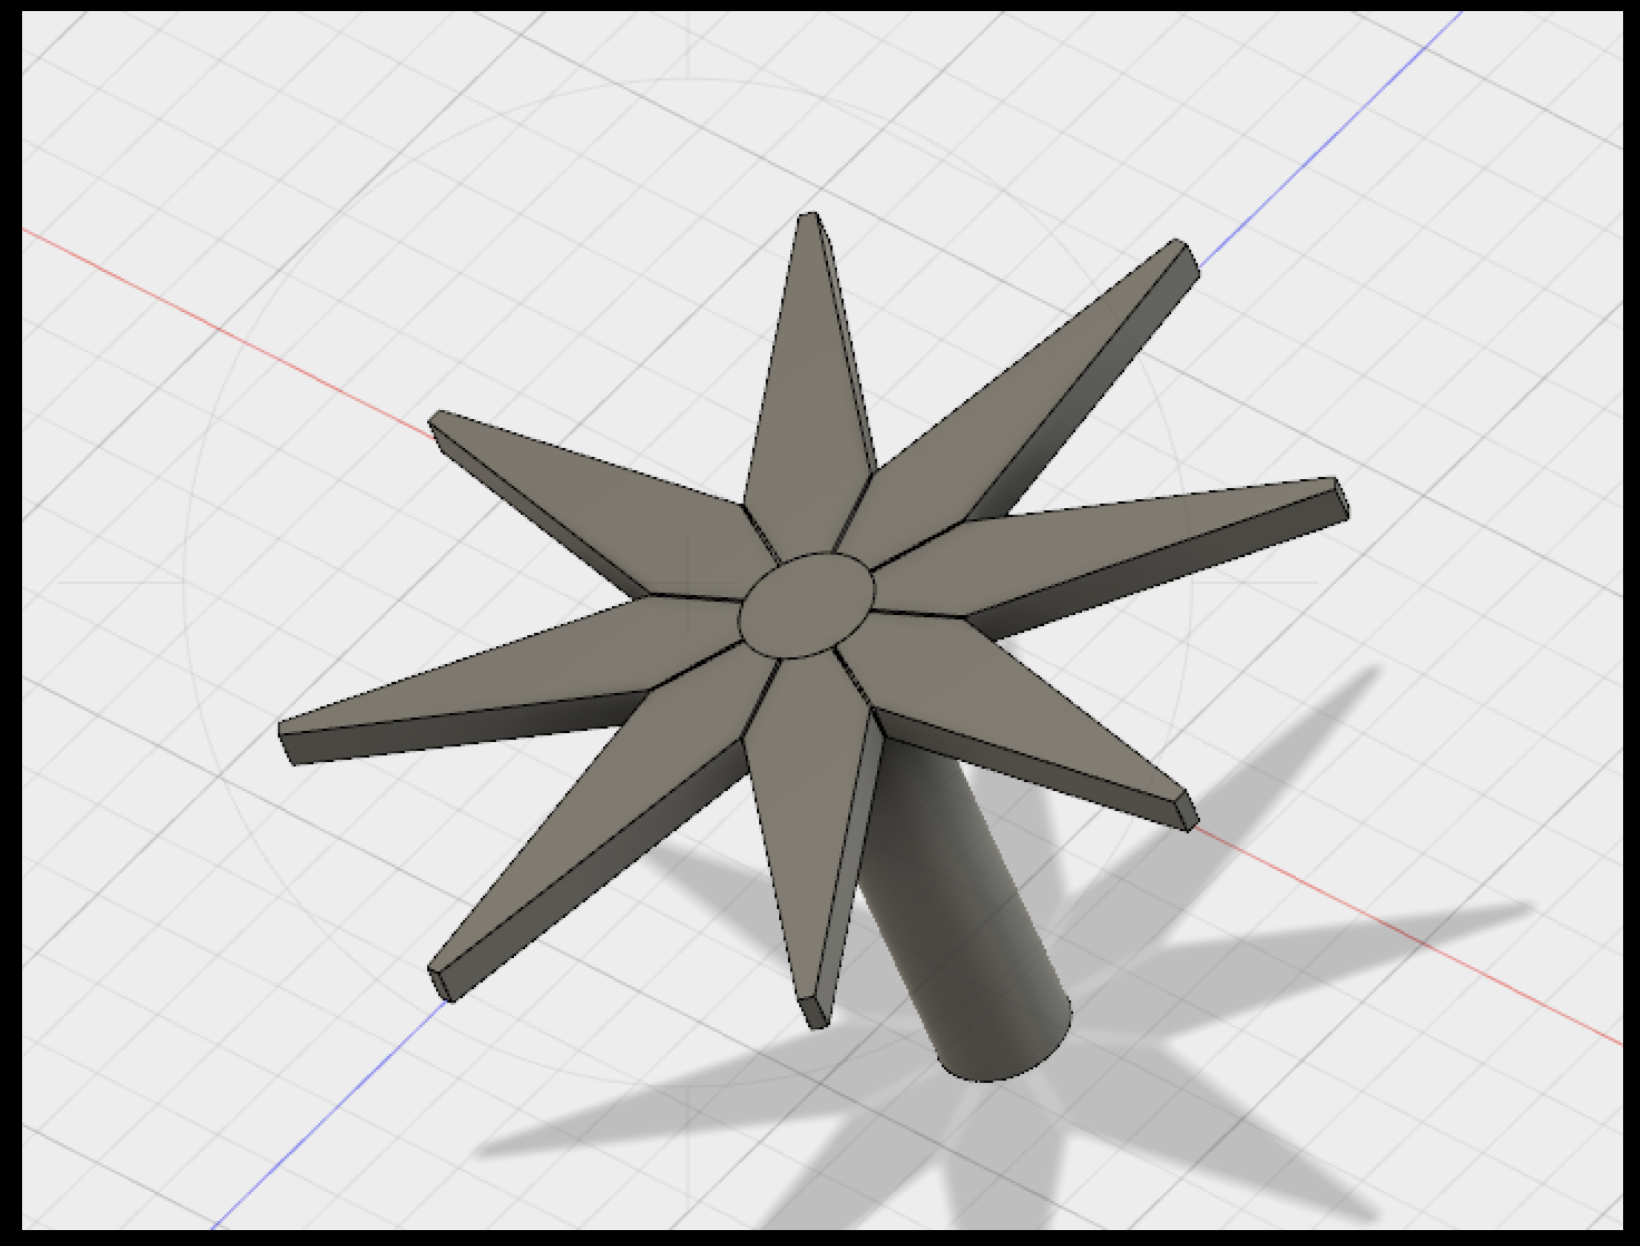
\includegraphics[width=0.8\linewidth]{ibfe-coral-model-fusion360.png}\\
{\tiny The coral polyp model drawn in Fusion 360 for the 2018 two-coral IBFE example (chapter 21).}
\end{column}
\end{columns}
\end{frame}

% 17
\begin{frame}{File formats you will meet}
\scriptsize
\begin{tabular}{@{}L{0.13\textwidth}L{0.44\textwidth}L{0.36\textwidth}@{}}
\toprule
Format & What it is & Where it goes\\
\midrule
STL & triangles only, no units, no connectivity (binary or text) & out of CAD and scanners; into meshers and repair tools\\
OBJ, PLY & triangles with normals, colors or texture; PLY is common for scans & scanners and photogrammetry; convert to STL for meshing\\
STEP, IGES & exact CAD solids (surfaces, not triangles) & between CAD programs; gmsh and Cubit can mesh them directly\\
MSH & gmsh's own format; version 2.2 text is what libMesh reads best & the mesh file of IBFE examples 05 and 10\\
Exodus (\code{.e}, \code{.ex2}) & the Sandia finite element format; Cubit writes it, IBFE reads and writes it & IBFE/08's meshes; every IBFE run's \code{output.ex2}\\
\code{.poly} & TetGen and Triangle input: points and boundary segments & 2D and 3D meshes made from an outline (chapter 18)\\
SVG & 2D vector drawing & MeshmerizeMe's input for IB2d and IBAMR points\\
\bottomrule
\end{tabular}
\vspace{2mm}
\begin{punchbox}
\small libMesh reads text files. A binary MSH stops IBAMR with \code{Unknown data format for mesh in Gmsh reader}, and an MSH 4 binary file is the gmsh default: save with \code{-format msh22} or choose ASCII in the export dialog (IBFE/05's README).
\end{punchbox}
\end{frame}

% 18
\begin{frame}{Why a surface needs repair}
\begin{columns}[T,onlytextwidth]
\begin{column}{0.5\textwidth}
A mesher wants a \al{closed, manifold} surface: every edge shared by exactly two triangles, no triangle crossing another, inside and outside well defined. Scans and downloads have:
\begin{itemize}
  \item holes and missing patches;
  \item floating fragments and duplicated vertices;
  \item self-intersections and inside-out normals;
  \item noise, and features far smaller than the grid will resolve;
  \item millions of triangles, more than any mesher needs.
\end{itemize}
\end{column}
\begin{column}{0.47\textwidth}
\begin{punchbox}
\small Bad surfaces make bad volume meshes, and bad meshes make bad simulations: very flat ``sliver'' tetrahedra deform wildly (IBFE/10's README shows J straying from 0.2 to 2.7 in them), and tiny elements force a tiny time step.
\end{punchbox}
\vspace{2mm}
\small Aim for a surface whose triangles are about the size of the fluid grid cell $\Delta x$ at the organism: finer features are invisible to the simulation and only cost time.
\end{column}
\end{columns}
\end{frame}

% 19
\begin{frame}{Tools for repair and smoothing}
\scriptsize
\begin{tabular}{@{}L{0.16\textwidth}L{0.45\textwidth}L{0.32\textwidth}@{}}
\toprule
Tool & Operations & Status (October 2026)\\
\midrule
Autodesk Meshmixer & Inspector (auto-repair), Make Solid, Smooth, Reduce, Remesh; the tool of the 2018--2024 courses & \al{no longer developed}; its web site now redirects to an Autodesk app listing. Keep a copy if you have one; otherwise use the tools below\\
Blender & 3D-Print Toolbox (checks), Remesh modifier (voxel size $\approx \Delta x$), Smooth, Decimate, Solidify, Boolean & free, \url{https://www.blender.org}\\
MeshLab & Close Holes, Remove Duplicates, Screened Poisson surface, Laplacian and Taubin smoothing, Quadric decimation & free, \url{https://www.meshlab.net}\\
Autodesk Fusion & Mesh workspace: Repair, Reduce, Smooth, Convert Mesh to a solid body & free for education\\
gmsh & Reclassify and Remesh an STL (Mesh $\to$ Reclassify 2D) & free, \url{https://gmsh.info}\\
\bottomrule
\end{tabular}
\vspace{1mm}
\begin{itemize}
  \item The operations are the same in every tool: repair (close, remove, fix normals), \al{remesh} to a uniform triangle size, \al{smooth}, \al{reduce} the count, export STL. Trelis and Bolt, the csimsoft meshers of the 2018 notes, became \al{Coreform Cubit} (next slides).
\end{itemize}
\end{frame}

% 20
\begin{frame}{The smoothing recipe, old and new}
\begin{columns}[T,onlytextwidth]
\begin{column}{0.5\textwidth}
\small\textbf{As done in Meshmixer (legacy, 2018--2024)}
\begin{enumerate}
  \item Import the STL; Analysis $\to$ Inspector, auto-repair all.
  \item Edit $\to$ Make Solid: a closed surface, with the ``solid accuracy'' set so that the cell size is about $\Delta x$.
  \item Sculpt $\to$ Smooth (brush) or Deform $\to$ Smooth (whole object).
  \item Edit $\to$ Reduce to the triangle count you want.
  \item Export STL (binary is fine for meshers; text for inspection).
\end{enumerate}
\textbf{The same in Blender}: a Remesh modifier (Voxel, size $\approx \Delta x$), applied; Smooth (or Corrective Smooth); Decimate; File $\to$ Export $\to$ STL.
\end{column}
\begin{column}{0.47\textwidth}
\centering
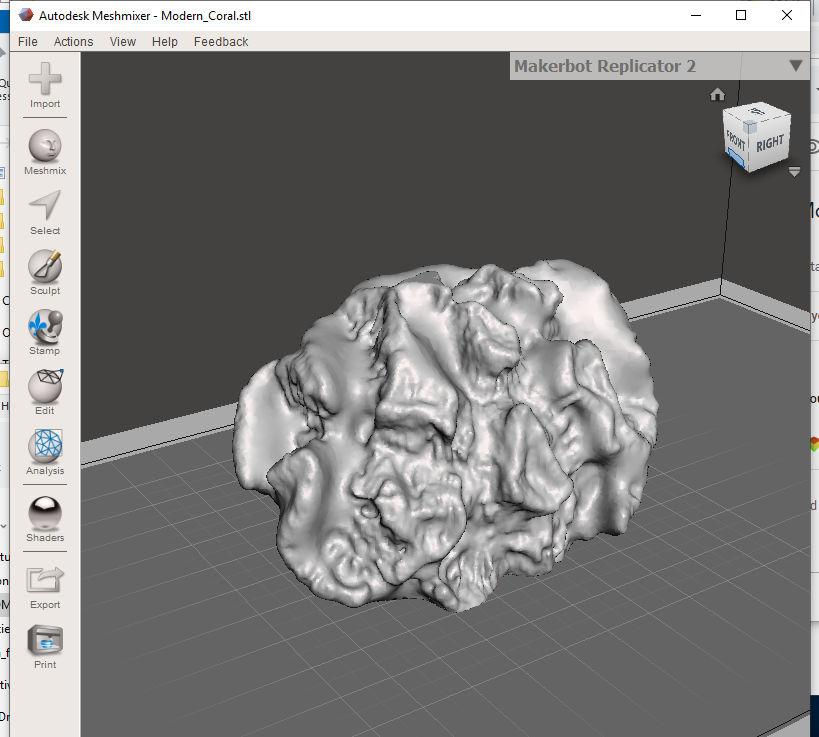
\includegraphics[width=0.85\linewidth]{cfd-coral-meshmixer.png}\\
{\tiny The scanned coral in Meshmixer after Make Solid and smoothing (2024 workshop). The original scan had holes and a rough surface.}
\end{column}
\end{columns}
\end{frame}

% 21
\begin{frame}[fragile]{From a surface to a volume mesh}
\begin{columns}[T,onlytextwidth]
\begin{column}{0.55\textwidth}
\small
\begin{itemize}
  \item \al{gmsh} (free): tetrahedra from a closed STL, a \code{.geo} script or a STEP file. Text format 2.2 is what IBFE reads.
  \item \al{Coreform Cubit}: tetrahedra \emph{and} hexahedra, Exodus output, a free Learn edition with a limit on mesh size; the successor of Trelis and Bolt. SALOME, TetGen (\code{.poly}) and Triangle (2D): chapter 18.
\end{itemize}
\begin{lstlisting}[style=geo,basicstyle=\ttfamily\tiny\color{BlackGray}]
// coral.geo: mesh a repaired STL with gmsh
Merge "coral_smooth.stl";
Surface Loop(1) = {1};  Volume(1) = {1};
Physical Volume("coral") = {1};
Mesh.CharacteristicLengthMax = 0.0005;  // about dx
\end{lstlisting}
\begin{lstlisting}[style=shell,basicstyle=\ttfamily\tiny\color{BlackGray}]
gmsh -3 -format msh22 coral.geo -o coral.msh
\end{lstlisting}
\end{column}
\begin{column}{0.43\textwidth}
\centering
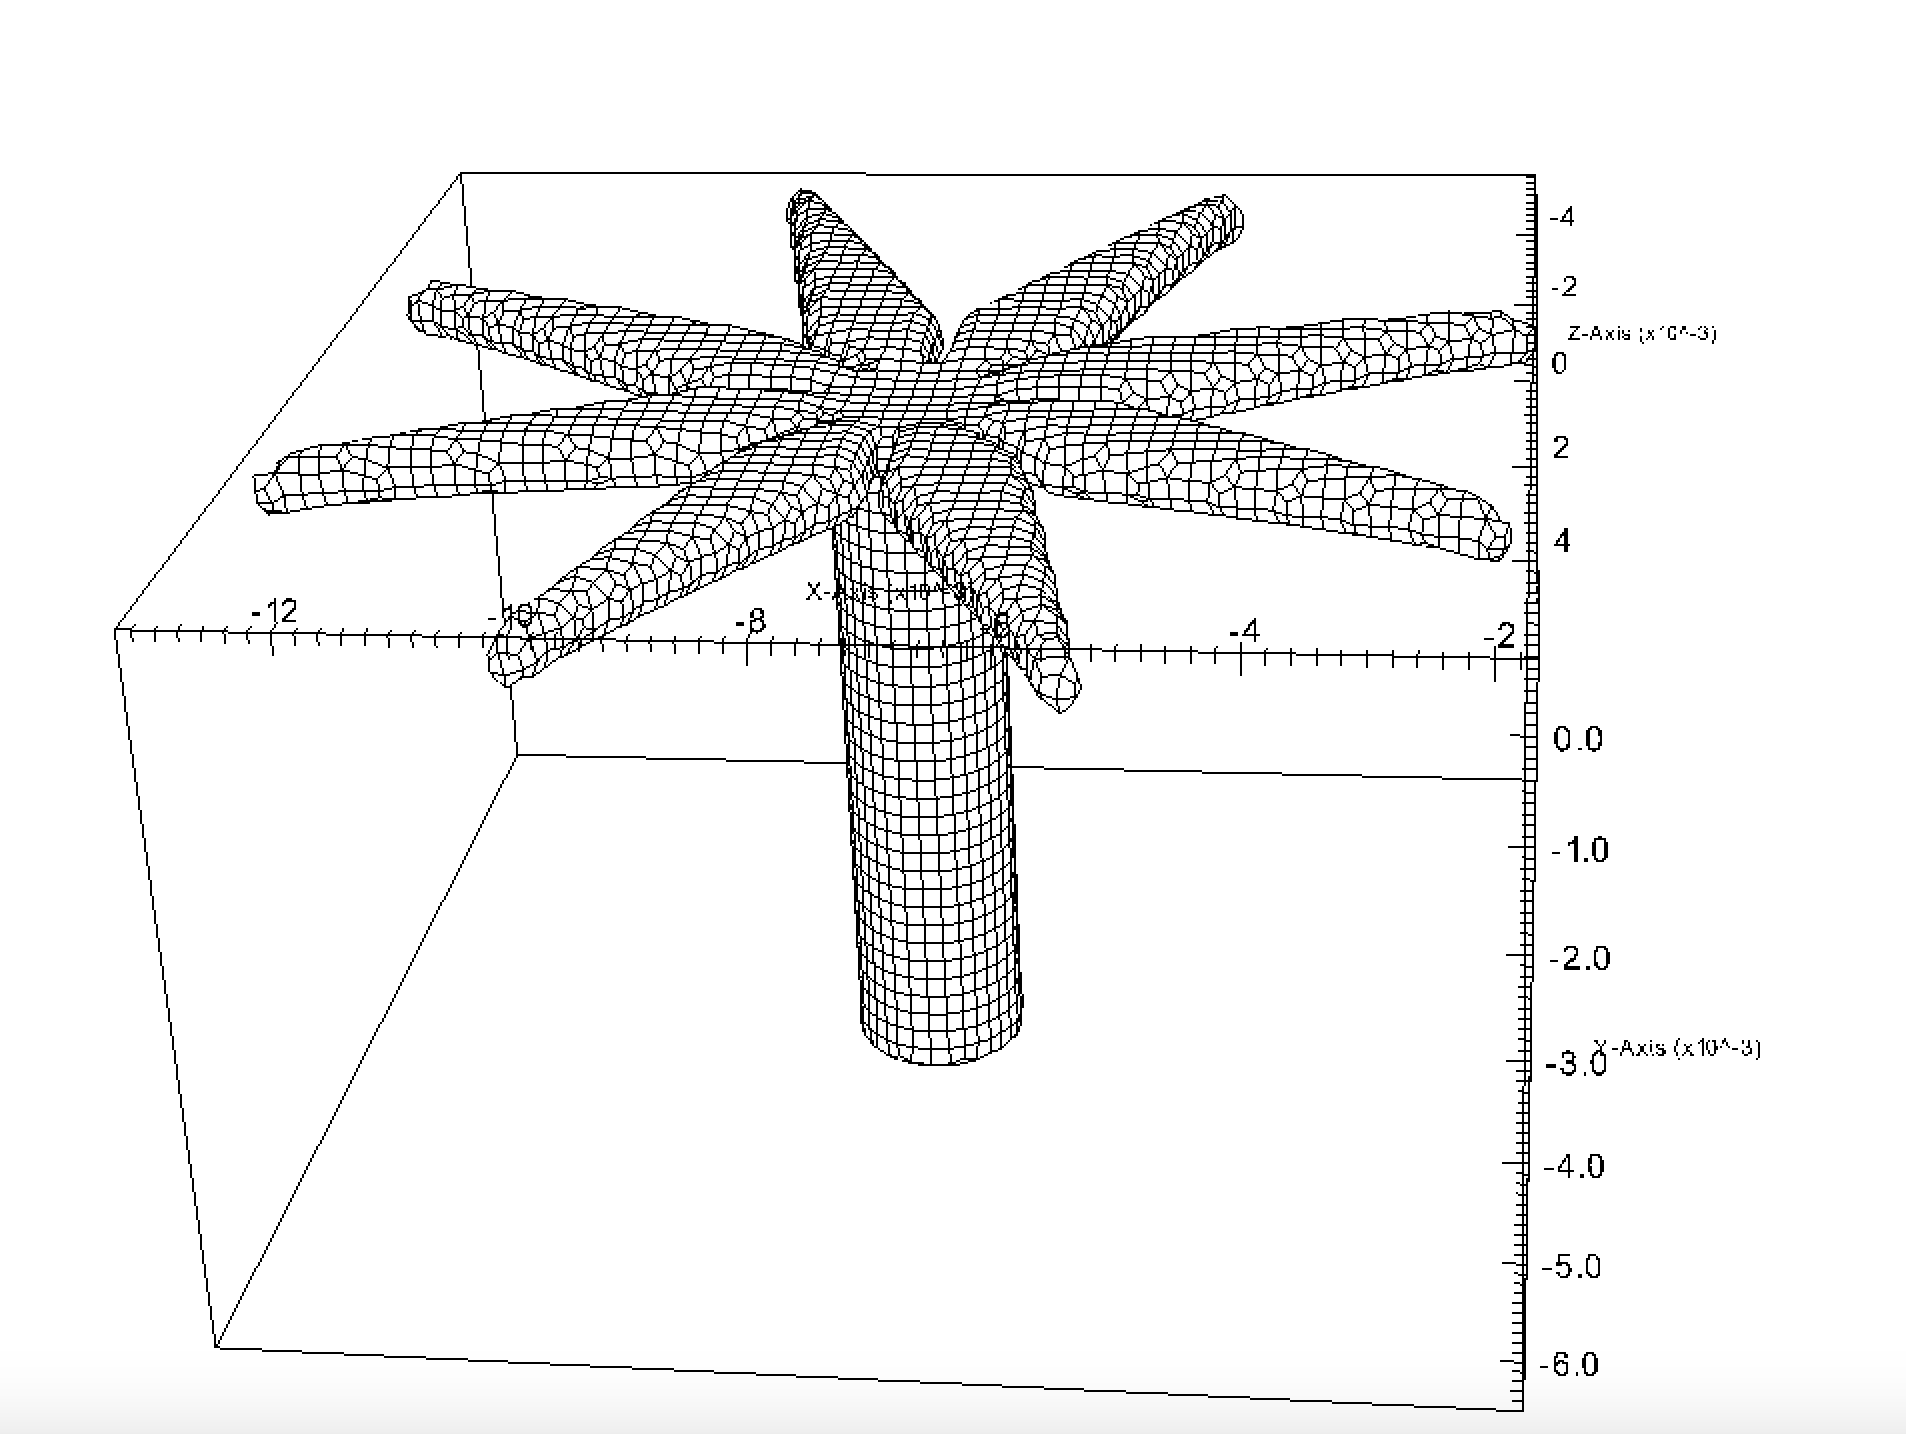
\includegraphics[width=0.72\linewidth]{ibfe-coral-hexmesh-bolt.png}\\
{\tiny The 2018 coral polyp meshed with hexahedra in Bolt (now Coreform Cubit), elements about one grid cell across.}
\begin{punchbox}
\small Element size $\approx \Delta x$ of the finest grid level: finer costs time and tiny time steps; coarser lets fluid leak through the solid (chapter 17).
\end{punchbox}
\end{column}
\end{columns}
\end{frame}

% 22
\begin{frame}{Checking a mesh before IBFE}
\begin{columns}[T,onlytextwidth]
\begin{column}{0.55\textwidth}
\footnotesize
\begin{enumerate}
  \item A \al{text} file: MSH 2.2 (or MSH 4 text) or Exodus.
  \item One \al{physical volume} (gmsh) or block (Cubit) holding the volume elements; once any physical group exists, gmsh saves only what is in groups (IBFE/05).
  \item Elements with \al{positive Jacobians}, or IBAMR stops (``the Jacobian of each element must be positive''); gmsh's Reverse mesh fixes an inverted surface.
  \item Element size about $\Delta x$; no slivers: gmsh's \emph{Optimize 3D} or \emph{Netgen optimize}, or remesh the surface first.
  \item Units and position matching \code{input3d}: measure the bounding box.
  \item A short run (\code{END\_TIME} a few steps) before the long one.
\end{enumerate}
\end{column}
\begin{column}{0.43\textwidth}
\begin{punchbox}
\small Chapter 18 shows each check in gmsh and in Cubit, and chapter 28 shows how to look at the mesh in VisIt before you run anything. IBFE/05's README lists the three most common mesh-file errors with IBAMR's exact messages.
\end{punchbox}
\vspace{1mm}
\small gmsh reports element quality (Tools $\to$ Statistics); elements below 0.05 on its scale are the slivers to fix.
\end{column}
\end{columns}
\end{frame}

% 23
\begin{frame}{2D geometries for IB2d and IBAMR}
\begin{columns}[T,onlytextwidth]
\begin{column}{0.55\textwidth}
\small The IB method needs \al{points along the boundary}, about half a grid cell apart, joined by springs, beams or target points (chapter 6). Ways to get them:
\begin{itemize}
  \item \al{Write them}: the MATLAB and Python generators in every example (an ellipse, a line, a row of circles) are 30-line scripts; copy and change one.
  \item \al{Draw them}: MeshmerizeMe turns an SVG drawing (Inkscape, Illustrator) into IB2d and IBAMR files (chapter 4f; Senter et al.\ 2021).
  \item \al{Trace them}: from a photograph with Inkscape's Trace Bitmap, then MeshmerizeMe.
  \item \al{Cut them}: a section through a 3D model (Blender or MeshLab) gives the outline of a 2D model.
\end{itemize}
\end{column}
\begin{column}{0.43\textwidth}
\begin{punchbox}
\small Whatever makes the points, check the spacing against $\Delta x$ (chapter 5) and look at the result before running: \code{test\_IB2d\_IBAMR\_Geometry.m} in \code{examples/support} (and its Python version) plots the points and springs of any structure file.
\end{punchbox}
\vspace{1mm}
{\scriptsize MeshmerizeMe: D. M. Senter et al., Bioinspiration \& Biomimetics 16:016008 (2021); \url{https://github.com/dmsenter89/MeshmerizeMe}.}
\end{column}
\end{columns}
\end{frame}

% 24
\begin{frame}{Visualization software}
\scriptsize
\begin{tabular}{@{}L{0.13\textwidth}L{0.21\textwidth}L{0.58\textwidth}@{}}
\toprule
Software & Cost, platforms & Notes\\
\midrule
\al{VisIt} & free; Linux, macOS, Windows & reads IBAMR's SAMRAI dumps and Exodus files directly, and IB2d's VTK files; scriptable in Python; runs client--server on a cluster. Used throughout Part V. \url{https://visit-dav.github.io/visit-website/}\\
ParaView & free; Linux, macOS, Windows & reads VTK and Exodus; the most common alternative; a similar client--server mode. \url{https://www.paraview.org}\\
Tecplot & license; Windows, Linux, macOS & common in engineering groups. \url{https://tecplot.com}\\
MATLAB, Python & & for numbers rather than pictures: forces, averages, convergence (chapters 11 and 33)\\
\bottomrule
\end{tabular}
\vspace{1mm}
\begin{itemize}
  \item VisIt's home moved from the LLNL web site to GitHub; the old link still redirects. Whichever tool you use, the first picture to make of a new mesh is the mesh itself, before any flow (chapter 28).
\end{itemize}
\end{frame}

% 25
\begin{frame}{A worked path: the scanned coral}
\begin{columns}[T,onlytextwidth]
\begin{column}{0.5\textwidth}
\small The 2024 workshop followed one coral from a scan to a flow:
\begin{enumerate}
  \item a scanned coral surface, with holes and noise (STL);
  \item Meshmixer: Make Solid, Smooth, Reduce (previous slides);
  \item a flow tank around it in a commercial code (the workshop's Parts 2 and 3, ANSYS Fluent and COMSOL: out of scope here);
  \item velocity and pressure fields around and through the branches.
\end{enumerate}
\vspace{1mm}
\small The same smoothed STL goes into gmsh (slide 21) and then into IBFE's flow tank (chapter 22, example IBFE/10), with tether points to hold it (chapter 19).
\end{column}
\begin{column}{0.47\textwidth}
\centering
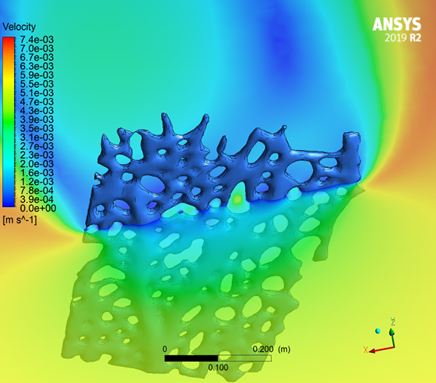
\includegraphics[width=0.66\linewidth]{cfd-coral-flow-ansys-2019.png}\\
{\tiny Velocity magnitude around the smoothed coral in a flow tank (ANSYS Fluent, 2019). The geometry work is the same for IBFE.}
\end{column}
\end{columns}
\end{frame}

% 26
\begin{frame}{Legacy tools and what replaced them}
\scriptsize
\begin{tabular}{@{}L{0.29\textwidth}L{0.64\textwidth}@{}}
\toprule
In the older notes & Now (checked October 2026)\\
\midrule
Meshmixer (2018--2024 courses) & no longer developed; Blender, MeshLab or Autodesk Fusion's mesh workspace\\
Trelis and Bolt (csimsoft, 2018) & Coreform Cubit, with a free Learn edition\\
Fusion 360 & Autodesk Fusion (renamed; still free for education)\\
cuIBM & archived; PetIBM is the Barba group's current code\\
NIH 3D Print Exchange (\code{3dprint.nih.gov}) & NIH 3D, \url{https://3d.nih.gov} (the old address redirects)\\
VisIt at \code{wci.llnl.gov} & \url{https://visit-dav.github.io/visit-website/} (the old address redirects)\\
FreeCAD at \code{freecadweb.org} & \url{https://www.freecad.org}\\
ANSYS & part of Synopsys since 2025; the products keep their names\\
Autodesk ReCap Photo for photogrammetry & still exists with education access; Meshroom and the phone apps are the free routes\\
\bottomrule
\end{tabular}
\vspace{2mm}
\small Every link in this chapter was opened in October 2026. Some sites block automatic checks and were opened by hand.
\end{frame}

% 27
\begin{frame}{What can go wrong}
\scriptsize
\begin{tabular}{@{}L{0.34\textwidth}L{0.59\textwidth}@{}}
\toprule
Symptom & Cause and fix\\
\midrule
The organism is 1000 times too big or too small & STL has no units; the exporter assumed millimeters. Scale the model, or set the box in \code{input3d} to match.\\
Nothing happens, or ``Jacobian \ldots negative'' at the first step & the mesh is not where the fluid box is, or it was moved with a coordinate mapping into a wall. Check the bounding box (IBFE/10's \code{TRANSLATE\_X} shows the mapping).\\
gmsh takes hours or runs out of memory & too many surface triangles; reduce the surface to about $\Delta x$ first.\\
``surface not closed'', ``self-intersecting'' from the mesher & repair the surface (slide 19); Make Solid or Remesh usually fixes both.\\
\code{Unknown data format for mesh in Gmsh reader} & a binary MSH; save as text, format 2.2 (IBFE/05).\\
``the Jacobian of each element must be positive'' & inverted elements; reverse the surface or run \code{fix\_orientation.py} (IBFE/05).\\
J far from 1 in a few elements; a tiny stable time step & slivers; Optimize 3D in gmsh, or remesh.\\
Fluid leaks through the solid & elements much larger than $\Delta x$; refine the mesh or coarsen the grid (chapter 17).\\
\bottomrule
\end{tabular}
\end{frame}

% 28
\begin{frame}{Summary}
\begin{enumerate}
  \item IB2d (2D, laptop) and IBAMR with IBFE (3D, cluster) are the codes of these notes; OpenFOAM and the commercial codes cover rigid, high-Re flows.
  \item Different codes and different meshes give different answers until the boundaries, the mesh and the run length are checked; report converged quantities.
  \item A 3D model comes from a download, a scan, photographs or CAD; draw a simplified organism in real units for your first simulation.
  \item Repair and smooth the surface to triangles about $\Delta x$ across (Blender, MeshLab or Fusion, now that Meshmixer is gone), then mesh it with gmsh or Coreform Cubit as a text MSH 2.2 or Exodus file.
  \item For 2D, write or draw the boundary points; check them before you run.
\end{enumerate}
\vspace{3mm}
\begin{homebox}
\small Next, chapter 2: installing IBAMR with autoibamr. Chapter 18 returns to the meshers in detail, with the examples IBFE/05, 08 and 10.
\end{homebox}
\end{frame}

% 29
\begin{frame}{What changed since the older course notes}
\begin{itemize}
  \item The 2024 workshop deck was a tour of software and links; this chapter adds the pipeline from organism to mesh, the checks before an IBFE run, and the 2D route.
  \item Meshmixer, used in every geometry lecture from 2018 to 2024, is no longer developed; the recipe is kept and translated to Blender and MeshLab.
  \item Trelis and Bolt (2018) are now Coreform Cubit; the NIH 3D Print Exchange is NIH 3D; VisIt's home moved; ANSYS belongs to Synopsys. Dead links were replaced and every link was checked.
  \item The 2022 CFD course's ANSYS pipeline (Fusion, Meshmixer, SpaceClaim, Workbench) and the workshop's COMSOL part are out of scope; their videos are listed in chapter 0.1.
  \item The 2022 ``3D repositories'' and ``photogrammetry'' tutorials are folded in here (their lists and tips), without their screenshots.
\end{itemize}
\end{frame}

% 30
\begin{frame}{References}
\scriptsize
\begin{itemize}
  \item O. Mesnard and L. A. Barba. Reproducible and replicable CFD: it's harder than you think. \emph{Computing in Science \& Engineering} 19(4):44--55, 2017. \url{https://arxiv.org/abs/1605.04339}
  \item R. J. Bomphrey, T. Nakata, N. Phillips and S. M. Walker. Smart wing rotation and trailing-edge vortices enable high frequency mosquito flight. \emph{Nature} 544:92--95, 2017.
  \item A. P. Hoover, N. W. Xu, B. J. Gemmell, S. P. Colin, J. H. Costello, J. O. Dabiri and L. A. Miller. Neuromechanical wave resonance in jellyfish swimming. \emph{PNAS} 118(11), 2021.
  \item D. M. Senter, D. R. Douglas, W. C. Strickland, S. G. Thomas, A. M. Talkington, L. A. Miller and N. A. Battista. A semi-automated finite difference mesh creation method for use with immersed boundary software IB2d and IBAMR. \emph{Bioinspiration \& Biomimetics} 16:016008, 2021.
  \item C. Geuzaine and J.-F. Remacle. Gmsh: a three-dimensional finite element mesh generator with built-in pre- and post-processing facilities. \emph{Int.\ J.\ Numer.\ Meth.\ Engng} 79:1309--1331, 2009. \url{https://gmsh.info}
  \item Coreform Cubit: \url{https://coreform.com/coreform-cubit/}. Blender: \url{https://www.blender.org}. MeshLab: \url{https://www.meshlab.net}. 3D Slicer: \url{https://www.slicer.org}.
  \item Sources: L. A. Miller, \emph{Software for Computational Fluid Dynamics, Part 1}, AIMEC--NSF Joint Workshop for the Model Species Cassiopea, 2024; the 2018 MATH 769 lecture on 3D target points; the 2020 IBFE lecture 5 tool list; the Spring 2022 CFD course tutorials on 3D repositories and photogrammetry.
\end{itemize}
\end{frame}

\end{document}
